\documentclass[a4paper,12pt]{article}

\usepackage[utf8]{inputenc}
\usepackage{amsmath, amssymb}
\usepackage{graphicx}
\usepackage{geometry}
\usepackage{hyperref}
\usepackage{setspace}
\usepackage{fancyhdr}
\usepackage{float}
\usepackage{lipsum}
\usepackage{listings}
\usepackage{xcolor}
\usepackage{xcolor-material}

\geometry{margin=1in}

\pagestyle{fancy}
\fancyhf{}
\fancyhead[L]{Laporan Final Sistem Tertanam}
\fancyhead[R]{\thepage}

\lstdefinestyle{mystyle}{
    backgroundcolor=\color{white},
    commentstyle=\color{green},
    keywordstyle=\color{magenta},
    numberstyle=\tiny\color{gray},
    stringstyle=\color{purple},
    basicstyle=\ttfamily\footnotesize,
    breakatwhitespace=false,
    breaklines=true,
    frame=single,
    captionpos=b,
    keepspaces=true,
    numbers=none,
    numbersep=10pt,
    showspaces=false,
    showstringspaces=false,
    showtabs=false,
    tabsize=2,
}

\lstset{style=mystyle}

\setlength{\parskip}{0.5em} % Adjust paragraph spacing
\setlength{\parindent}{0pt} % Remove paragraph indentation

\begin{document}
\begin{titlepage}
    \centering
    \vspace*{1cm}
    {\Large \textbf{Laporan Final \textit{Game PingPong} pada \textit{Dotmatrix Display}}}
    \vfill
    \vspace{2cm}

    
\includegraphics[width=0.4\textwidth]{./images/logo.png}
    \vfill

    \vspace{1cm}
    \begin{onehalfspace}
    \textbf{Dosen Pengampu}\\
    Eko Pramunanto, S.T. M.T.

    \vspace{1cm}

    \textbf{Disusun Oleh:}\\
    Muhammad Haekal Muhyidin Al-Araby\\
    5024221004\\
    Sistem Tertanam - A
    \end{onehalfspace}

    \vfill

    \textbf{DEPARTEMEN TEKNIK KOMPUTER\\
    FAKULTAS TEKNOLOGI ELEKTRO DAN INFORMATIKA CERDAS\\
    INSTITUT TEKNOLOGI SEPULUH NOPEMBER\\2024}
\end{titlepage}

\section{Gambaran Umum}
Pingpong atau tenis meja adalah salah satu olahraga yang dimainkan 2 orang yang saling berlawanan.
Untuk mendapat skor pemain harus memasukkan bola ke daerah lawan. Bola digerakkan dengan paddle. Pemain dapat
service, smash, maupun menangkis bola.

Project ini adalah implementasi dari pingpong ke dalam dotmatrix display dimana
player dapat mengendalikan paddle dengan slide potentiomenter dan smash dengan menekan button.
smash akan membuat bola bergerak lurus dan bertambah cepat.

Untuk memenangkan permainan Player harus mendapatkan skor lebih atau sama dengan 11 dan memiliki keunggulan 2 poin
dari lawan. Bila keunggulan tersebut tidak dimiliki maka permainan akan berlanjut terus menerus hingga keduanya mendapatkan skor 15
yang akan berakhir seri.

\section{Komponen}
\subsection{Normally Close Switch}
Saklar yang yang tertutup pada kondisi normal dan terbuka ketika ditekan. Dengan memanfaatkan pull-up internal
pada pin GPIO ESP32 dan menyambungkan ujung lainnya ke ground kita dapat mendapatkan nilai 1 ketika ditekan.
Pada project ini switch ini dimanfaatkan untuk player dapat melakukan smash saat ditekan.

\subsection{Slide Potentiometer}
Potentiometer jenis ini mengubah resistansi pada rangkaian dengan menggunakan mekanisme geser. Karena sifatnya
yang dapat menghasilkan data analog biasa digunakan untuk mengatur parameter suatu device dengan akurasi yang lebih
tinggi. Pada ESP32 kita dapat membaca nilai dari potentio meter ini dengan menggunakan pin ADC pada ESP32.
Pin ADC pada ESP32 dapat membaca nilai tegangan dengan rentang 0 - 3.3v setelah itu maka esp akan menunjukkan
nilai maksimum. Resolusi ADC dari ESP32 adalah dari rentang 0 - 12 dimana semakin tinggi resolusi akan semakin akurat namun
semakin berat juga pada performa. Pada project ini saya memilih 3 sebagai resolusi karena kita hanya membutuhkan
nilai 0 - 8. Karena hanya terdapat 8 pixel pada dotmatrix vertikal.

\subsection{Led DotMatrix 8x32}
Dotmatrix MAX7219 adalah modul untuk mengendalikan display dotmatrix 8x8 sebanyak 4 buah. Chip yang digunakan mampu
mengendalikan seluruh pixel pada dotmatrix. Informasi dikirimkan secara serial. Dan menyebar ke seluruh dotmatrix.
Led ini biasa digunakan untuk running text dan game interaktif.

\subsection{ESP32}
ESP32 adalah Microcontroller yang berfungsi sebagai pengendali utama sistem. ESP32 dapat menerima input analog
maupun digital. Lalu dapat mengeluarkan output digital melalui pin GPIO. ESP32 pada project ini diprogram
untuk menerima input dari Slide Potentiometer dan Normally Close Switch lalu memberikan keluaran pada 2 device
yaitu LED Dotmatrix dan Buzzer Pasif. Keluaran pada LED Dotmatrix berupa data digital yang dikirim secara serial
sedangkan pada buzzer berupa PWM.

\section{Desain Sistem}
\subsection{Rangkaian Skematik}
\begin{figure}[H]
    \centering
    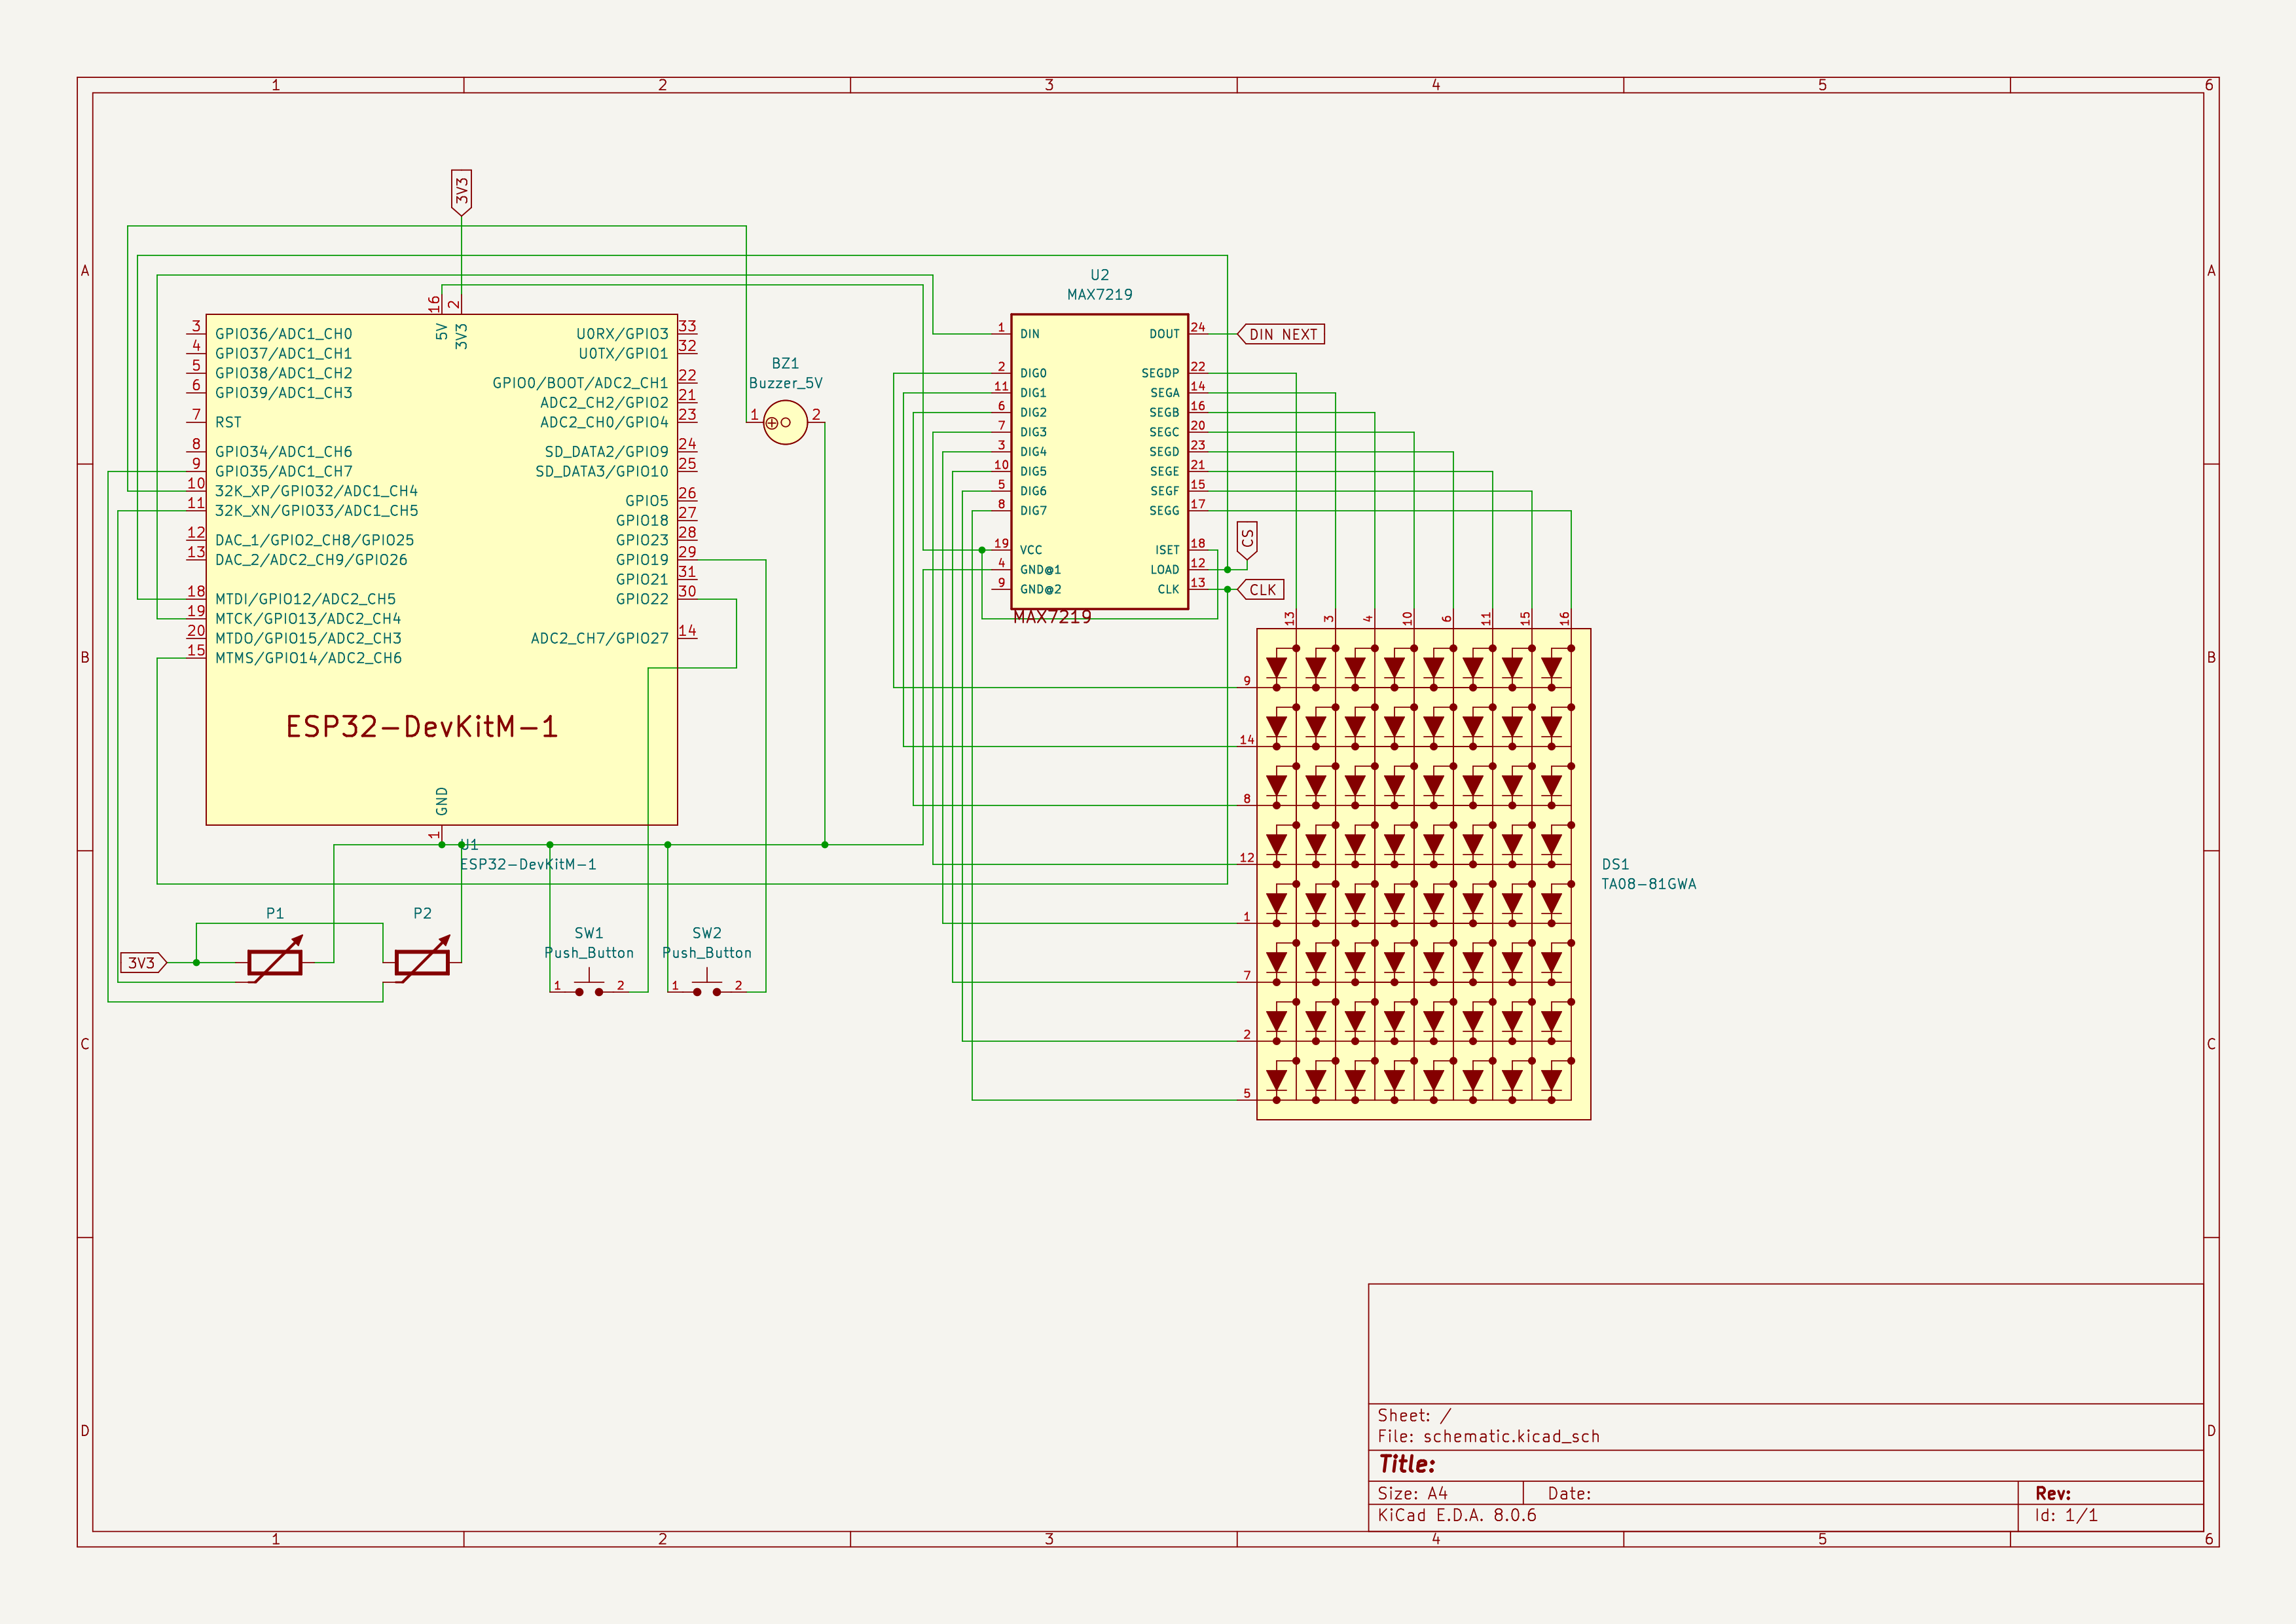
\includegraphics[width=1\textwidth]{images/schematic.png}
    \label{fig:schematic}
    \caption{Schematic}
\end{figure}
\subsection{Pemilihan Komponen}
\begin{enumerate}
    \item Potensiometer adalah slide potentiometer dengan resistansi variabel 220k ohm. Pemilihan ini dilakukan karena
        220 k ohm adalah nilai yang tepat dimana tidak terlalu rendah sehingga menghasilkan noise maupun terlalu tinggi
        sehingg tidak kompatibel dengan impedansi ESP32
    \item Normally Close Switch digunakan karena input smash adalah salah satu button yang pastinya akan
        sering ditekan sehingga dengan penggunaan komponen ini kerusakan akibat penggunaan diminimalkan.
\end{enumerate}

\subsection{Desain Game}
\begin{figure}[h!]
    \centering
    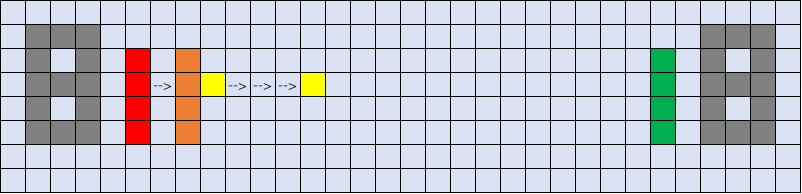
\includegraphics[width=1\textwidth]{images/desain_game.png}
    \label{fig:desaingame}
    \caption{Desain Game}
\end{figure}
\subsubsection{Mekanisme dan Peraturan Game}
\begin{enumerate}
    \item Game memiliki 2 player yang dapat digerakkan dengan slide potentiometer
    \item Bola memiliki kecepatan konstan
    \item Bola akan memantul saat menabrak pembatas ataupun player
        \begin{enumerate}
            \item Ketika bola mengenai pembatas bola akan memantul secara diagonal dengan mempertahankan gerakan horizontal
                dan membalik gerakan vertikal.
            \item Ketika bola mengenai player pada bagian tengah bola akan memantul secara lurus dan membalik
                gerakan horizontallnya
            \item Ketika bola mengenai player pada bagian atas bola akan memantul ke atas.
            \item Ketika bola mengenai player pada bagian bawah bola akan memantuk ke bawah.
        \end{enumerate}
    \item Bila bola melewati daerah player maka player lainnya akan mendapatkan skor 1.
    \item Player dapat melakukan smash.
        \begin{enumerate}
            \item Smash akan menggerakkan player 2 blok ke depan.
            \item Bila saat smash player mengenai bola, bola akan bergerak lurus dengan kecepatan tinggi
                ke arah lawan.
            \item Durasi smash adalah 0.2 detik
            \item Smash memiliki durasi cooldown 1 detik dimana setelah smash player tidak dapat melakukan smash lagi hingga cooldown berakhir.
            \item Ketika smash bola memiliki kemungkinan untuk melewati player dan memberikan
                skor kepada lawan.
        \end{enumerate}
    \item Player yang kebobolan akan mendapatkan kesempatan untuk melakukan service.
        \begin {enumerate}
            \item Saat service bola akan mengikuti gerakan player.
            \item Player dapat melakukan service dengan menekan tombol smash.
        \end {enumerate}
    \item Pemain yang mendapatkan skor di atas 11 dengan selisih 2 dari lawan memenangkan permainan
    \item Game akan berakhir imbang ketika kedua pemain mencapai 15 poin
\end{enumerate}
\subsubsection{Fitur}
\begin{enumerate}
    \item Permainan diiringi dengan musik yang berasal dari Buzzer.
        \begin{enumerate}
            \item terdapat 2 musik yaitu Tetris Theme dan Mario Theme
            \item Tetris Theme diputar saat menu awal muncul, pemain mencetak skor, dan saat permainan berakhir.
            \item Mario Theme saat permainan berlangsung. Mario Theme dipilih karena nadanya yang cukup tenang
                sehingga tidak mengganggu konsentrasi pemain.
        \end{enumerate}
    \item Tiap event seperti mencetak skor dan kemenangan mempunyai animasi tersendiri
    \begin{enumerate}
        \item Saat pemain mencetak skor akan ditampilkan animasi Text dari arah player yang mencetak skor.
        \item Saat salah satu pemain menang akan tampil juga animasi Text dari player yang menang.
        \item Ketika imbang animasi akan muncul dari arah bawah.
    \end{enumerate}
\end{enumerate}
\section{Implementasi}
\subsection{Hardware}
Seperti yang terlihat pada schematic, rangkaian menggunakan ESP32 yang terhubung pada IC MAX7219 dimana CS
terhubung pada pin D12, DIN pada D13 dan clock pada D14. Lalu VCC menggunakan pin 5V
pada modul terdapat 4 IC MAX7219 yang saling terhubung secara seri.

Untuk input dari push button pada 1 pin dihubungkan pada ground dan 1 nya dihubungkan pada GPIO 19 dan 22 yang masing
masing berfungsi untuk input smash button dari player 1 dan 2 berturut-turut. Selanjutnya untuk input gerakan player menggunakan
slide potentiometer yang di kedua ujung dihubungkan pad VCC 3.3 V dan Ground. Lalu output dari potentiometer
berturut-turut dihubungkan ke GPIO 33 dan 35 untuk mengendalikan gerakan player 1 dan player 2.

Untuk buzzer sendiri digunakan buzzer pasif yang dihubungkan ke GPIO 32 dan GROUND.

Wiring digunakan menggunakan kabel yang disolder pada pcb untuk menjamin konektivitas.

Input dari player 1 dan player 2 dipisahkan dan dihubungkan dengan kabel agar dapat dimainkan dengan jarak yang cukup.

\subsection{Software}
\subsubsection{Alur Program}
\begin{enumerate}
    \item Program dimulai dengan inisialisasi Global Variabel yang terdapat pada global.hpp dan global.cpp, variabel tersebut
        akan digunakan pada keseluruhan program. Dimana variabel bila memungkinkan akan menggunakan keyword static sehingga akan sama. Sedangkan
        yang tidak memungkinkan menggunakan keyword static akan menggunakan keyword extern dan didefine pada global.gpp
    \item Program lalu menjalankan fungsi Setup pada device untuk melakukan inisiasi dan setup pada device MAX7019
        menggunakan library MD\_Parola dan MD\_MAX72xx
    \item Setelah itu program akan menjalankan intro yang berisi animasi dan text nama dan nrp.
    \item Lalu program akan menampilkan menu yang bertuliskan "PRESS ANY BUTTON TO START...", dimana program
        akan menunggu user untuk menekan tombol apapun. Pada saat ini program juga akan memutar musik tetris theme.
    \item Sebelum program memasuki loop utama music akan diganti terlebih dahulu ke mario theme dan player 1 diberi kesempatan service.
    \item Program memasuki main loop
    \item Program akan memeriksa apakah memasuki loop setelah game berahir atau tidak bila iya akan diberi delay 100.
    \item Music akan diputar pada tiap loop dengan memanggil fungsi Play pada class MusicPlayer
    \item Program akan melakukan update posisi dan memeriksa input pada tiap loop.
    \item Setiap 100ms program akan melakukan update display dengan clear display lalu memanggil fungsi Draw pada
        class Player dan Ball. juga melakukan RenderScore untuk skor Player 1 dan Player 2.
    \item Setelah itu program akan memeriksa kondisi kemenangan pada permainan. Dan menampilkan animasi yang sesua dengan kondisi
        yang terpenuhi.
    \item Permainan akan berulang ketika salah satu button ditekan.
\end{enumerate}
\subsection{Source Code dan Penjelasan}
\subsubsection{Main Program}
Pada bagian ini program utama akan dijalankan dengan alur yang sudah dijelaskan pada subsection alur code.
\lstinputlisting[language=C++, caption={main.cpp}]{../src/main.cpp}
\subsubsection{Display Functionality}
Display dilakukan dengan 2 metode yaitu menggunakan MD\_Parola untuk menampilkan animasi text dan MD\_MAX72xx untuk menampilkan
pixel secara manual. Pada bagian ini program akan menginsialisasi device dotmatrix dengan parameter dan pin yang telah ditentukan.
\lstinputlisting[language=C++, caption={device.hpp}]{../include/device.hpp}
\lstinputlisting[language=C++, caption={device.cpp}]{../src/device.cpp}
Class Vector2 digunakan untuk merepresentasikan koordinat kartesian pada koordinat Dotmatrix dan untuk melakukan fungsi Draw
dimana fungsi Draw akan memanggil fungsi setPoint pada MD\_MAX72xx untuk menyalakan pixel pada koordinat vector tersebut.
\lstinputlisting[language=C++, caption={vector2.hpp}]{../include/vector2.hpp}
\lstinputlisting[language=C++, caption={vector2.cpp}]{../src/vector2.cpp}
Pada bagian ini didefinisikan fungsi intro yang berisi pola-pola untuk ditampilkan pada intro permainan. Dengan
memanggil fungsi dari MD\_MAX72xx untuk menyalakan pixel dan mematikan pixel secara manual sesuai dengan pola yang sudah ditentukan
\lstinputlisting[language=C++, caption={animation.hpp}]{../include/animation.hpp}
\lstinputlisting[language=C++, caption={animation.cpp}]{../src/animation.cpp}
Pada bagian fungsi ini array Vector2 yang merepresentasikan posisi masing masing segment pada display yang digunakan
untuk menampilkan score. Terdapat juga array dari binary representation untuk segment yang dinyalakan dan dimatikan pada angkat tersebut.
Untuk menampilkan skor program akan mengiterasi masing masing segment dan binary reporesentationnya dan menyalakan pixel sesuai dengan nilainya.
\lstinputlisting[language=C++, caption={score.hpp}]{../include/score.hpp}
\lstinputlisting[language=C++, caption={score.cpp}]{../src/score.cpp}
\subsubsection{Player Functionality}
Pada class Player terdapat fungsi check input dan draw serta constructor class itu sendiri. Pada constructor
program akan setup pin yang ada pada parameter sebagai input pull-up.

Selanjutnya pada fungsi Draw program akan mengaktifkan pixel pada vector2 posisi dia dan 1 diatas dan 1 dibawah.

Lalu pada fungsi CheckInput program akan membaca nilai analog dari pin yang terhubung pada potentiometer, pin
ditentukan saat inisialisasi class. Posisi player akan dipindahkan berdasarkan nilai tersebut. Posisi player dibatasi
agar tidak melebihi layar.

Pada fungsi ini juga akan dicek apakah player sudah melakukan service atau smash dan apakah sudah 0.2 detik
bila iya player akan dikembalikan ke posisi semula.

Pada fungsi ini juga dibaca smash input dan dicek apakah sudah melewati cooldown atau tidak. Bila iya maka player akan smash.
\lstinputlisting[language=C++, caption={player.hpp}]{../include/player.hpp}
\lstinputlisting[language=C++, caption={player.cpp}]{../src/player.cpp}
\subsubsection{Ball Functionality}
Pada class Ball terdapat constructor,update, fungsi hit check, dan score check.
pada constructor dimana saat class diinisiasi bola akan berapada pada player 1 dan player 1 dapat melakukan service.

Pada fungsi Update program akan memeriksa apakah sudah melewati periode update belum. Periode update ditentukan dengan membagi 75 / update rate.
dimana pada kondisi normal update rate adalah 1 yang berarti bola akan diupdate per 75ms. Semakin cepat update rate maka hal ini akan memengaruhi
kecepatan bola. Fungsi ini akan memanggil HitCheck ScoreCheck secara berurutan dan menambahkan move vector pada vector position untuk
mengupdate posisi bola.

Pada fungsi HitCheck program akan mengecek apakah bola terkena pembatas atau player. Bila terkena pembatas hanya akan membalikkan nilai y dari move vector.
Sedangkan bila terkena Player bola akan memantuk tergantung dari dimana bola tersebut mengenainya.

Pada fungsi ScoreCheck program akan mengecek apakah bola masuk ke daerah player atau tidak dan memberikan skor pada player yang berhasil memasukkan.
\lstinputlisting[language=C++, caption={ball.hpp}]{../include/ball.hpp}
\lstinputlisting[language=C++, caption={ball.cpp}]{../src/ball.cpp}
\subsubsection{Music Functionality}
Fungsionalitas utama lagu dikendalikan oleh class MusicPlayer dimana pada MusicPlayer terdapat beberapa
fungsi Switch, Start, dan Play lalu constructor dari kelas itu sendiri. Pada saat class diinisiasi akan attach ledc ke pin 32. Hal ini
untuk menginsialisasi pin 32 untuk PWM. resolusi yang digunakan adalah 12 bit.

Fungsi Switch digunakan untuk mengganti lagu yang sedang dimainkan dengan mengganti variabel song. Lalu memanggil
fungsi start untuk memulai lagu. Pada fungsi start index akan menjadi 0 dan pin akan mengoutputkan notes pertama dari lagu.

Fungsi Play akan memainkan lagu dengan cara mengecek apakah sudah melewati durasi notes atau tidak.
durasi tiap notes ditentukan dengan membagi 1000 dengan absolut tempo dari lagu. Bila tempo lagu adalah negatif dimana merepresentasikan
tempo titik. Maka durasi akan dikali 1.5. Ketika sudah melewati durasi maka akan memainkan note selanjutnya.
\lstinputlisting[language=C++, caption={music.hpp}]{../include/music.hpp}
Bagian ini berisi lagu lagu yang dapat dimainkan.
\lstinputlisting[language=C++, caption={song.hpp}]{../include/song.hpp}
Bagian ini berisi nada yang dapat dioutputkan
\lstinputlisting[language=C++, caption={song.hpp}]{../include/note.hpp}
\subsubsection{Global Variable}
\lstinputlisting[language=C++, caption={global.hpp}]{../include/global.hpp}
\lstinputlisting[language=C++, caption={global.cpp}]{../src/global.cpp}
\subsection{Hasil}
\begin{figure}[h!]
    \centering
    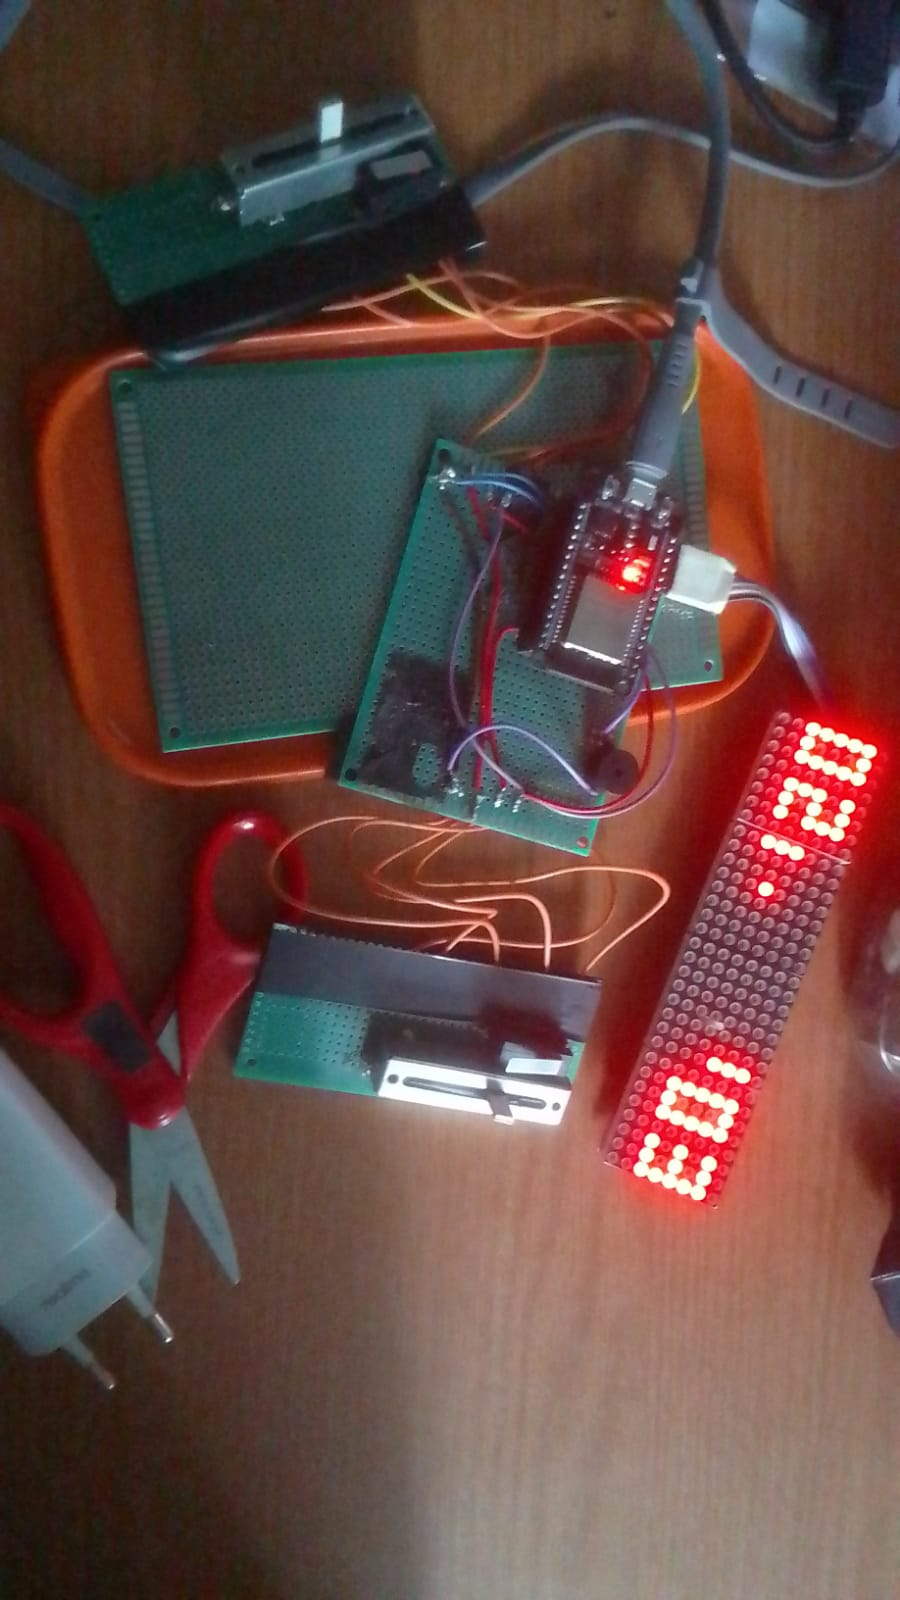
\includegraphics[width=0.5\textwidth]{./images/no-package.jpeg}
    \caption{Hasil tanpa package}
\end{figure}
\begin{figure}[h!]
    \centering
    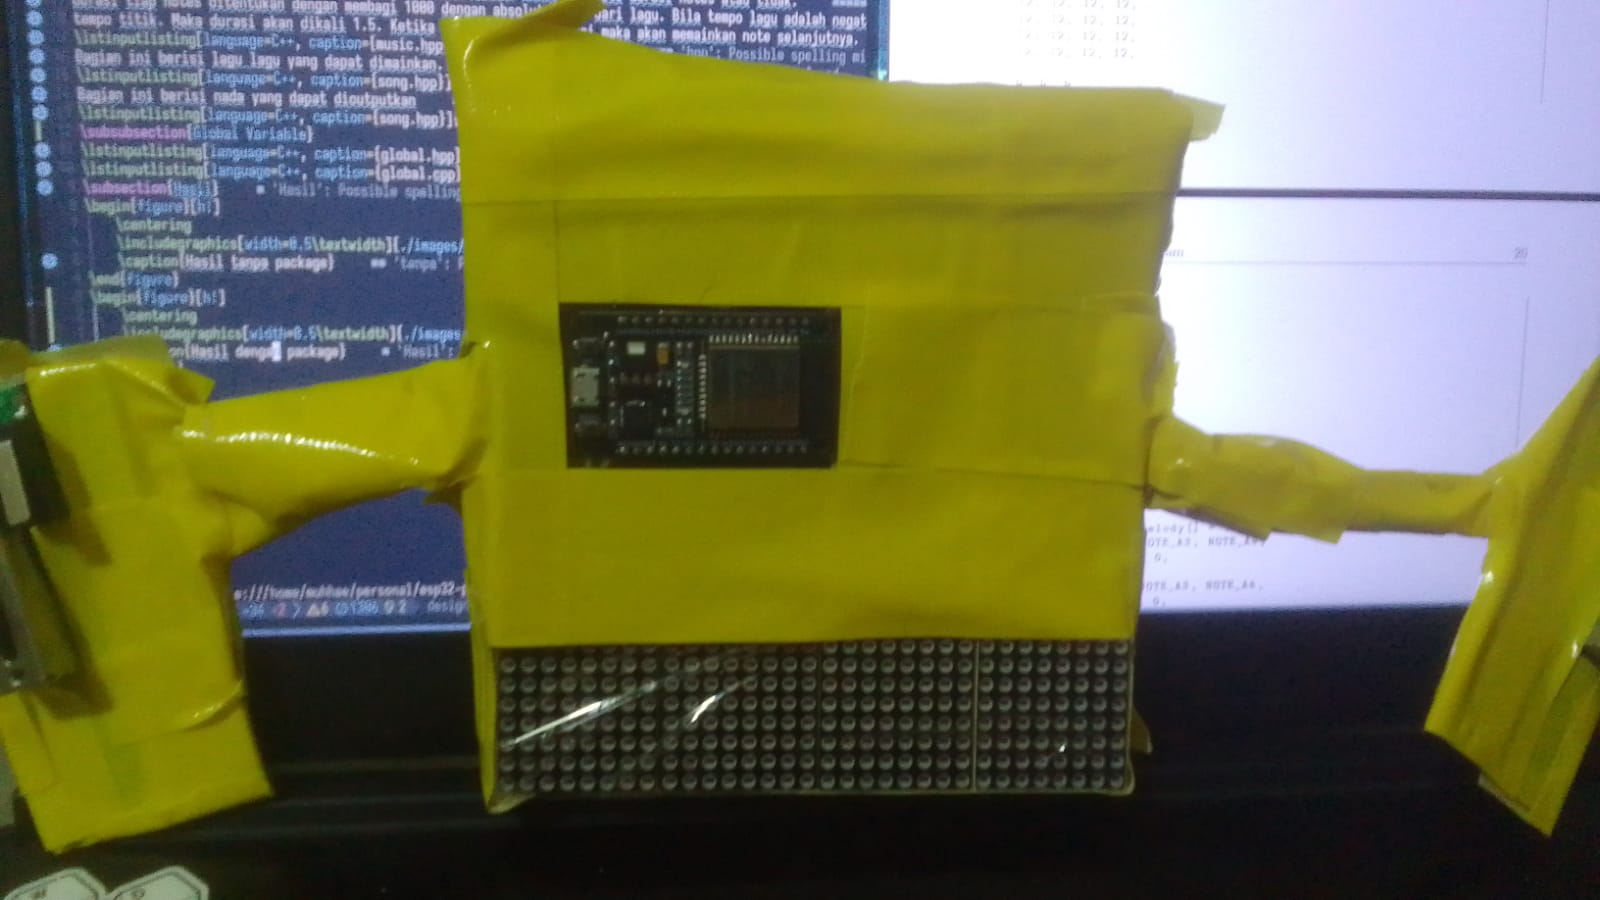
\includegraphics[width=0.5\textwidth]{./images/with_package.jpeg}
    \caption{Hasil dengan package}
\end{figure}
\end{document}
